%package list
\documentclass{article}
\usepackage[top=3cm, bottom=3cm, outer=3cm, inner=3cm]{geometry}
\usepackage{multicol}
\usepackage{graphicx}
\usepackage{url}
\usepackage{hyperref}
\usepackage{array}
\newcolumntype{x}[1]{>{\centering\arraybackslash\hspace{0pt}}p{#1}}
\usepackage{natbib}
\usepackage{pdfpages}
\usepackage{multirow}
\usepackage[normalem]{ulem}
\useunder{\uline}{\ul}{}
\usepackage{svg}
\usepackage{xcolor}
\usepackage{listings}
\lstdefinestyle{ascii-tree}{
    literate={├}{|}1 {─}{--}1 {└}{+}1 
  }
\lstset{basicstyle=\ttfamily,
  showstringspaces=false,
  commentstyle=\color{red},
  keywordstyle=\color{blue}
}
%\usepackage{booktabs}
\usepackage{caption}
\usepackage{subcaption}
\usepackage{float}
\usepackage{array}

% Comment
\usepackage{verbatim}

\newcolumntype{M}[1]{>{\centering\arraybackslash}m{#1}}
\newcolumntype{N}{@{}m{0pt}@{}}


%%%%%%%%%%%%%%%%%%%%%%%%%%%%%%%%%%%%%%%%%%%%%%%%%%%%%%%%%%%%%%%%%%%%%%%%%%%%
%%%%%%%%%%%%%%%%%%%%%%%%%%%%%%%%%%%%%%%%%%%%%%%%%%%%%%%%%%%%%%%%%%%%%%%%%%%%
\newcommand{\itemEmail}{rzapata@unsa.edu.pe}
\newcommand{\itemStudent}{Reyser Julio Zapata Butron}
\newcommand{\itemCourse}{Tecnología de Objetos}
\newcommand{\itemCourseCode}{1703240}
\newcommand{\itemSemester}{VI}
\newcommand{\itemUniversity}{Universidad Nacional de San Agustín de Arequipa}
\newcommand{\itemFaculty}{Facultad de Ingeniería de Producción y Servicios}
\newcommand{\itemDepartment}{Departamento Académico de Ingeniería de Sistemas e Informática}
\newcommand{\itemSchool}{Escuela Profesional de Ingeniería de Sistemas}
\newcommand{\itemAcademic}{2024 - B}
\newcommand{\itemInput}{03 octubre 2024}
\newcommand{\itemOutput}{09 octubre 2024}
\newcommand{\itemPracticeNumber}{03}
\newcommand{\itemTheme}{C++ Herencia, Polimorfismo, Qt}
\newcommand{\itemPracticeDuration}{02 horas}
%%%%%%%%%%%%%%%%%%%%%%%%%%%%%%%%%%%%%%%%%%%%%%%%%%%%%%%%%%%%%%%%%%%%%%%%%%%%
%%%%%%%%%%%%%%%%%%%%%%%%%%%%%%%%%%%%%%%%%%%%%%%%%%%%%%%%%%%%%%%%%%%%%%%%%%%%

\usepackage[english,spanish]{babel}
\usepackage[utf8]{inputenc}
\AtBeginDocument{\selectlanguage{spanish}}
\renewcommand{\figurename}{Figura}
\renewcommand{\refname}{Referencias}
\renewcommand{\tablename}{Tabla} %esto no funciona cuando se usa babel
\AtBeginDocument{%
	\renewcommand\tablename{Tabla}
}

\usepackage{fancyhdr}
\pagestyle{fancy}
\fancyhf{}
\setlength{\headheight}{30pt}
\renewcommand{\headrulewidth}{1pt}
\renewcommand{\footrulewidth}{1pt}
\fancyhead[L]{\raisebox{-0.2\height}{
\includegraphics[width=3cm]{img/logo_episunsa.png}}}
\fancyhead[C]{\fontsize{7}{7}\selectfont	\itemUniversity \\ \itemFaculty \\ \itemDepartment \\ \itemSchool \\ \textbf{\itemCourse}}
\fancyhead[R]{\raisebox{-0.2\height}{
\includegraphics[width=1.2cm]{img/logo_abet}}}
\fancyfoot[L]{\itemStudent}
\fancyfoot[C]{\itemCourse}
\fancyfoot[R]{Página \thepage}

% Estilos del Código
\usepackage{listings}
\usepackage{color, colortbl}
\definecolor{dkgreen}{rgb}{0,0.6,0}
\definecolor{gray}{rgb}{0.5,0.5,0.5}
\definecolor{codebackground}{rgb}{89, 0.97, 0.90}
\definecolor{tablebackground}{rgb}{0.8, 0, 0}

\lstset{
  language=C++,                  
  basicstyle=\ttfamily\footnotesize,
  keywordstyle=\color{blue},     
  commentstyle=\color{dkgreen},    
  stringstyle=\color{red},       
  backgroundcolor= \color{codebackground},
  numbers=left,                  
  numberstyle=\tiny\color{gray},
  stepnumber=1,                  
  numbersep=5pt,                
  showspaces=false,              
  showstringspaces=false,      
  showtabs=false,                
  frame=single,                  
  captionpos=b,                  %
}

\begin{document}
	\vspace*{10px}
	
	\begin{center}	
		\fontsize{17}{17} \textbf{ Informe de Laboratorio \itemPracticeNumber}
	\end{center}

 %% TABLA %%
 
	\centerline{\textbf{\Large Tema: \itemTheme}}

	\begin{flushright}
		\begin{tabular}{|M{2.5cm}|N|}
			\hline 
			\rowcolor{tablebackground}
			\color{white} \textbf{Nota}  \\
			\hline 
			     \\[30pt]
			\hline 			
		\end{tabular}
	\end{flushright}	

	\begin{table}[H]
		\begin{tabular}{|x{4.7cm}|x{4.8cm}|x{4.8cm}|}
			\hline 
			\rowcolor{tablebackground}
			\color{white} \textbf{Estudiante} & \color{white}\textbf{Escuela}  & \color{white}\textbf{Asignatura}   \\
			\hline 
			{\itemStudent \par \itemEmail} & \itemSchool & {\itemCourse \par Semestre: \itemSemester \par Código: \itemCourseCode}     \\
			\hline 			
		\end{tabular}
	\end{table}		
	
	\begin{table}[H]
		\begin{tabular}{|x{4.7cm}|x{4.8cm}|x{4.8cm}|}
			\hline 
			\rowcolor{tablebackground}
			\color{white}\textbf{Laboratorio} & \color{white}\textbf{Tema}  & \color{white}\textbf{Duración}   \\
			\hline 
			\itemPracticeNumber & \itemTheme & \itemPracticeDuration   \\
			\hline 
		\end{tabular}
	\end{table}
	
	\begin{table}[H]
		\begin{tabular}{|x{4.7cm}|x{4.8cm}|x{4.8cm}|}
			\hline 
			\rowcolor{tablebackground}
			\color{white}\textbf{Semestre académico} & \color{white}\textbf{Fecha de inicio}  & \color{white}\textbf{Fecha de entrega}   \\
			\hline 
			\itemAcademic & \itemInput &  \itemOutput  \\
			\hline 
		\end{tabular}
	\end{table}

 %%% REPOSITORIO DE GITHUB %%%
\section{Repositorio de Github}
	\begin{itemize}
		\item Repositorio de Github donde se encuentra el actual laboratorio \\
		\url{https://github.com/ReyserLynnn/tec-obj-lab-c-24b/tree/main/laboratorio03/src}

        \item Repositorio de Github donde se encuentran los laboratorios del curso\\
		\url{https://github.com/ReyserLynnn/tec-obj-lab-c-24b.git}
	\end{itemize}
 

 %% CONTENIDO %%
\section{Ejercicios}
En los siguientes ejercicios, se presentará código, captura de ejecución y una explicación en general por cada ejercicio.\\

    \subsection{Ejercicio 1}
        \begin{itemize}
            \item Modificar el ejercicio 01 (rectángulo) para que funcione en la memoria dinámica. Los miembros de la clase deben ser punteros, las instancias en el main deben cargarse en memoria dinámica, el constructor debe crear la instancia en la memoria dinámica. Utilizar punteros inteligentes.

        \end{itemize}  
        
        \lstinputlisting[language=C++, caption={rectangulo.h}, numbers=left]{src/ejercicio1/rectangulo.h}

        \lstinputlisting[language=C++, caption={rectangulo.cpp}, numbers=left]{src/ejercicio1/rectangulo.cpp}

        \lstinputlisting[language=C++, caption={main.cpp}, numbers=left]{src/ejercicio1/main.cpp}
        

        \textbf{Ejecución del ejercicio}
        \begin{figure}[H]
        	\centering
         	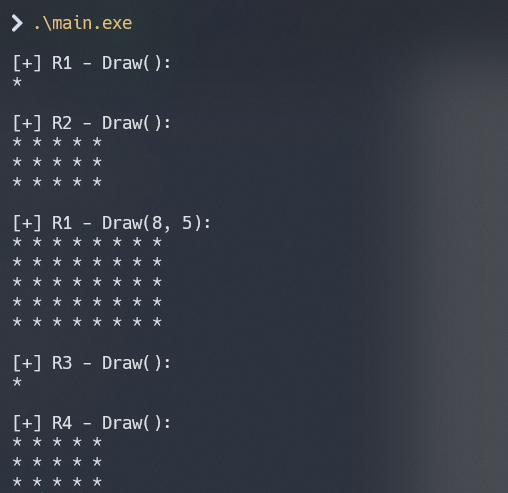
\includegraphics[width=0.8\textwidth,keepaspectratio]{img/ejercicio1.png}
        \end{figure}

        \textbf{Análisis del código:} \\\\
        El código implementa la clase \texttt{Rectangulo}, que usa \texttt{unique\_ptr} para gestionar dinámicamente la memoria de atributos como \texttt{width}, \texttt{height}, \texttt{temperatura}, \texttt{presion} y \texttt{humedad}. Se incluyen tres constructores y un método para dibujar el rectángulo.
        
        Se ofrecen tres constructores:
        \begin{itemize}
            \item \texttt{Rectangulo()} - Crea un rectángulo de 1x1 con valores predeterminados.
            \item \texttt{Rectangulo(USHORT w, USHORT h)} - Inicializa un rectángulo con dimensiones personalizadas.
            \item \texttt{Rectangulo(const Rectangulo \&R)} - Copia profunda de otro objeto \texttt{Rectangulo}.
        \end{itemize}
        
        \texttt{Draw()} asigna valores a \texttt{temperatura}, \texttt{presion} y \texttt{humedad} antes de llamar a la versión sobrecargada que dibuja el rectángulo con las dimensiones proporcionadas.
        
        El uso de \texttt{unique\_ptr} asegura la gestión eficiente de memoria, liberándola automáticamente cuando los objetos son destruidos, evitando fugas de memoria.
        

    \subsection{Ejercicio 2}
        \begin{itemize}
            \item Modificar el ejercicio 02 (time) para que funcione en memoria dinámica. Los miembros de la clase deben ser punteros, las instancias en el main deben cargarse en memoria dinámica, el constructor debe crear la instancia en la memoria dinámica. Utilizar punteros inteligentes.
        \end{itemize}  
        
        \lstinputlisting[language=C++, caption={time.h}, numbers=left]{src/ejercicio2/time.h}

        \lstinputlisting[language=C++, caption={time.cpp}, numbers=left]{src/ejercicio2/time.cpp}
        
        \lstinputlisting[language=C++, caption={main.cpp}, numbers=left]{src/ejercicio2/main.cpp}

        \textbf{Ejecución del ejercicio} \\\\
        \begin{figure}[H]
        	\centering
         	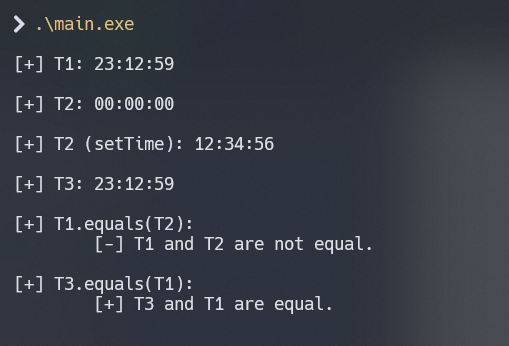
\includegraphics[width=0.8\textwidth,keepaspectratio]{img/ejercicio2.png}
        \end{figure}

        \textbf{Análisis del código:}  \\\\
        El código implementa una clase \texttt{Time} que gestiona la hora usando punteros inteligentes \texttt{unique\_ptr} para las horas, minutos y segundos, asegurando una correcta gestión de la memoria.
        
        La clase define dos constructores:
        \begin{itemize}
            \item \texttt{Time(USHORT h=0, USHORT m=0, USHORT s=0)} - Inicializa la hora con los valores proporcionados o por defecto a 00:00:00.
            \item \texttt{Time(const Time \&T)} - Constructor de copia que realiza una copia profunda de otro objeto \texttt{Time}.
        \end{itemize}
        
        \begin{itemize}
            \item \texttt{void setTime(USHORT h, USHORT m, USHORT s)} - Establece una nueva hora.
            \item \texttt{void printTime()} - Imprime la hora en formato \texttt{hh:mm:ss}, con ceros a la izquierda.
            \item \texttt{bool equals(const Time \&T)} - Compara si dos objetos \texttt{Time} tienen la misma hora.
        \end{itemize}
        
        El uso de \texttt{unique\_ptr} para gestionar los atributos garantiza que no haya fugas de memoria, ya que estos punteros gestionan automáticamente el ciclo de vida de la memoria asignada. \\
        
        En \texttt{main()}, se crean varios objetos \texttt{Time} utilizando tanto el constructor por defecto como el constructor parametrizado. Se comparan las horas de los objetos usando el método \texttt{equals()} y se imprimen los resultados de la comparación.\\
        
        
        \subsection{Ejercicio 3}
        \begin{itemize}
            \item Modificar el ejercicio 02 (time) para que funcione en memoria dinámica. Los miembros de la clase deben ser punteros, las instancias en el main deben cargarse en memoria dinámica, el constructor debe crear la instancia en la memoria dinámica. Utilizar punteros inteligentes.
        \end{itemize}  
        
        \lstinputlisting[language=C++, caption={Nodo.h}, numbers=left]{src/ejercicio3/Nodo.h}
        
        \lstinputlisting[language=C++, caption={Lista.h}, numbers=left]{src/ejercicio3/Lista.h}

        \lstinputlisting[language=C++, caption={Lista.cpp}, numbers=left]{src/ejercicio3/Lista.cpp}
        
        \lstinputlisting[language=C++, caption={main.cpp}, numbers=left]{src/ejercicio3/main.cpp}

        \textbf{Ejecución del ejercicio} \\\\
        \begin{figure}[H]
        	\centering
         	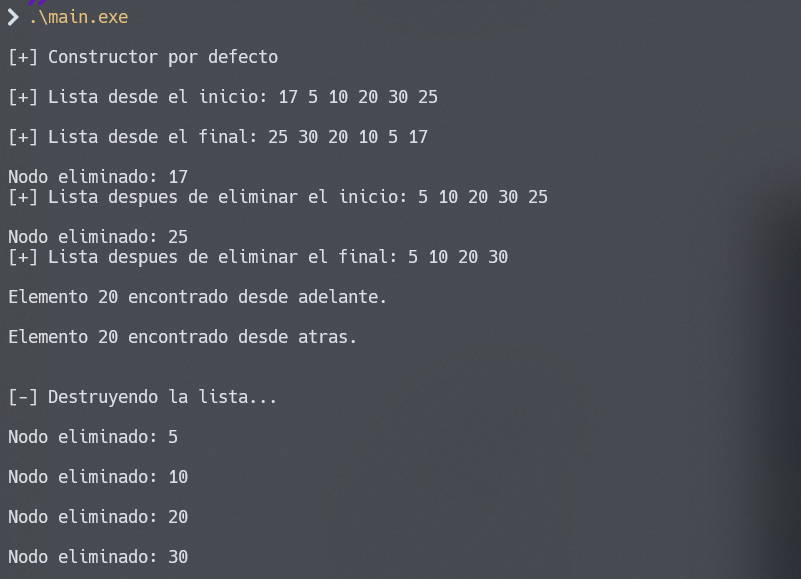
\includegraphics[width=0.8\textwidth,keepaspectratio]{img/ejercicio3.png}
        \end{figure}

        \textbf{Análisis del código:}  \\\\
        El código implementa una lista doblemente enlazada mediante las clases \texttt{Nodo} y \texttt{Lista}, proporcionando métodos para insertar, eliminar, buscar e imprimir elementos desde ambos extremos de la lista.
        
        La clase \texttt{Nodo} representa un nodo de la lista, compuesto por:
        \begin{itemize}
            \item \texttt{int valor} - Almacena el valor del nodo.
            \item \texttt{Nodo *siguiente} - Apunta al siguiente nodo.
            \item \texttt{Nodo *anterior} - Apunta al nodo anterior.
        \end{itemize}
        El constructor inicializa los punteros a \texttt{nullptr} y el destructor imprime un mensaje cuando se elimina un nodo.
        
        La clase \texttt{Lista} gestiona las operaciones de la lista mediante los punteros \texttt{cabeza} y \texttt{cola}, que apuntan al primer y último nodo, respectivamente.
        
        \begin{itemize}
            \item \texttt{insertarInicio(int valor)} - Inserta un nuevo nodo al principio de la lista.
            \item \texttt{insertarFinal(int valor)} - Inserta un nuevo nodo al final de la lista.
        \end{itemize}
        
        \begin{itemize}
            \item \texttt{eliminarInicio()} - Elimina el nodo al principio de la lista.
            \item \texttt{eliminarFinal()} - Elimina el nodo al final de la lista.
        \end{itemize}
        Ambos métodos manejan correctamente la eliminación de nodos, ajustando los punteros \texttt{cabeza} y \texttt{cola} cuando es necesario.
        
        \begin{itemize}
            \item \texttt{buscarDesdeAdelante(int valor)} y \texttt{buscarDesdeAtras(int valor)} - Buscan un nodo desde el inicio o el final de la lista.
            \item \texttt{imprimeDesdeAdelante()} e \texttt{imprimeDesdeAtras()} - Imprimen los valores de los nodos desde el inicio o el final de la lista.
        \end{itemize}
        
        El método \texttt{destruyeLista()} recorre toda la lista, eliminando los nodos para evitar fugas de memoria.
        
        Se realizó una implementación robusta de una lista doblemente enlazada, con métodos claros para su manipulación, incluyendo inserciones, eliminaciones y búsqueda eficiente en ambos sentidos de la lista.
        


        \subsection{Ejercicio 4}
        \begin{itemize}
            \item Implementar en C++ un Binary Expression Tree que pueda resolver operaciones matemáticas suma y multiplicación (usar clases y punteros).
        \end{itemize}  
        
        \lstinputlisting[language=C++, caption={Nodo.h}, numbers=left]{src/ejercicio4/Nodo.h}

        \lstinputlisting[language=C++, caption={NodoNumero.h}, numbers=left]{src/ejercicio4/NodoNumero.h}

        \lstinputlisting[language=C++, caption={NodoNumero.cpp}, numbers=left]{src/ejercicio4/NodoNumero.cpp}

        \lstinputlisting[language=C++, caption={NodoOperacion.h}, numbers=left]{src/ejercicio4/NodoOperacion.h}

        \lstinputlisting[language=C++, caption={NodoNumero.cpp}, numbers=left]{src/ejercicio4/NodoNumero.cpp}

        \lstinputlisting[language=C++, caption={NodoOperacion.h}, numbers=left]{src/ejercicio4/NodoOperacion.h}

        \lstinputlisting[language=C++, caption={analizador.cpp}, numbers=left]{src/ejercicio4/analizador.cpp}
        
        \lstinputlisting[language=C++, caption={main.cpp}, numbers=left]{src/ejercicio4/main.cpp}

        \textbf{Ejecución del ejercicio} \\\\
        \begin{figure}[H]
        	\centering
         	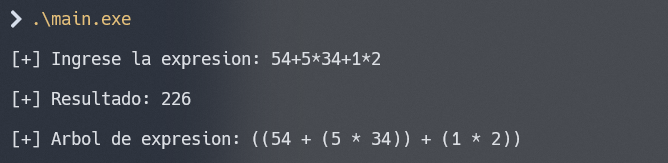
\includegraphics[width=0.8\textwidth,keepaspectratio]{img/ejercicio4_1.png}
        \end{figure}

        \begin{figure}[H]
        	\centering
         	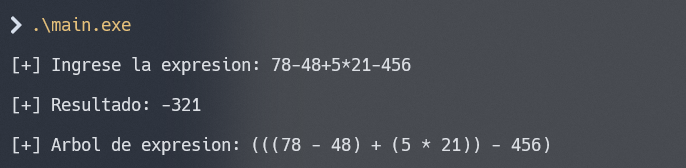
\includegraphics[width=0.8\textwidth,keepaspectratio]{img/ejercicio4_2.png}
        \end{figure}

        \begin{figure}[H]
        	\centering
         	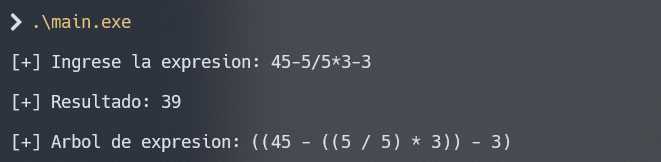
\includegraphics[width=0.8\textwidth,keepaspectratio]{img/ejercicio4_3.png}
        \end{figure}

        \textbf{Análisis del código:}  \\\\
        El programa desarrollado crea un Árbol de Expresiones Binarias, que permite evaluar operaciones matemáticas básicas (\texttt{+}, \texttt{-}, \texttt{*}, \texttt{/}) y generar una representación en notación infija de la expresión. Se compone de las siguientes clases y componentes principales:
        
        La clase abstracta \texttt{Nodo} define la interfaz básica para los nodos del árbol, que incluye dos métodos virtuales puros:
        \begin{itemize}
            \item \texttt{evaluar()} - Devuelve el valor calculado del nodo.
            \item \texttt{imprimir()} - Imprime el contenido del nodo.
        \end{itemize}
        Esta clase sirve como base para los nodos de tipo número y operación.
        
        Derivada de la clase \texttt{Nodo}, esta clase representa un nodo hoja que contiene un valor numérico. Implementa los métodos \texttt{evaluar()} para devolver el valor almacenado y \texttt{imprimir()} para mostrarlo.
        
        Esta clase también hereda de \texttt{Nodo}, y se utiliza para representar operaciones binarias (\texttt{+}, \texttt{-}, \texttt{*}, \texttt{/}). Contiene:
        \begin{itemize}
            \item \texttt{operador} - Un carácter que representa la operación.
            \item \texttt{hijoIzquierdo} y \texttt{hijoDerecho} - Punteros únicos a los nodos hijos, que pueden ser otros nodos de operación o número.
        \end{itemize}
        El método \texttt{evaluar()} realiza la operación entre los valores evaluados de los hijos, mientras que \texttt{imprimir()} muestra la expresión en notación infija, envolviendo la operación entre paréntesis.
        
        El \texttt{Analizador} procesa una expresión matemática representada como cadena y construye el árbol de expresiones correspondiente. Para ello, utiliza tres funciones:
        \begin{itemize}
            \item \texttt{parseExpresion()} - Procesa términos separados por sumas o restas.
            \item \texttt{parseTermino()} - Procesa factores separados por multiplicaciones o divisiones.
            \item \texttt{parseNumero()} - Extrae un número de la cadena de entrada.
        \end{itemize}
        El árbol se construye recursivamente al identificar los operadores y agrupar los operandos en subárboles.
        
        El programa principal solicita al usuario que ingrese una expresión. El analizador crea el árbol de la expresión, lo evalúa y luego imprime la expresión en notación infija.
        
        \begin{verbatim}
        [+] Ingrese la expresion: 3+5*2
        [+] Resultado: 13
        [+] Arbol de expresion: (3 + (5 * 2))
        \end{verbatim}

\section{Cuestionario}
        \subsection{Buscar y explicar sobre sobrecarga versus polimorfismo en C++. Proponer ejemplos.}
            \subsubsection{Sobrecarga}
            La sobrecarga de funciones permite declarar múltiples funciones con el mismo nombre pero diferentes parámetros, y se resuelve en tiempo de compilación. Ejemplo:
            
            \begin{verbatim}
            #include <iostream>
            
            void imprimir(int x) {
                std::cout << "Entero: " << x << std::endl;
            }
            void imprimir(double x) {
                std::cout << "Decimal: " << x << std::endl;
            }
            
            int main() {
                imprimir(5);    // Llama a la función con int
                imprimir(3.14); // Llama a la función con double
            }
            \end{verbatim}
            
            \subsubsection{Polimorfismo}
            El polimorfismo se refiere a la capacidad de clases derivadas de sobrescribir métodos de una clase base, y se resuelve en tiempo de ejecución, usando funciones virtuales. Ejemplo:
            
            \begin{verbatim}
            #include <iostream>
            
            class Animal {
            public:
                virtual void sonido() const { std::cout << "Sonido genérico\n"; }
            };
            
            class Perro : public Animal {
            public:
                void sonido() const override { std::cout << "El perro ladra\n"; }
            };
            
            int main() {
                Animal* a = new Perro();
                a->sonido();  // Llama a la versión de Perro
                delete a;
            }
            \end{verbatim}
            
            \subsubsection{Diferencias}
            - La sobrecarga ocurre en tiempo de compilación y se basa en la firma de la función.
            - El polimorfismo ocurre en tiempo de ejecución y depende del tipo real del objeto.

        \subsection{Buscar información de punteros inteligente. Poner ejemplos.} 
            \subsubsection{std::unique\_ptr}
            Es un puntero inteligente que posee un único propietario. El recurso se libera cuando el puntero es destruido o transferido. Ejemplo:
            
            \begin{verbatim}
            #include <iostream>
            #include <memory>
            
            int main() {
                std::unique_ptr<int> ptr = std::make_unique<int>(42);
                std::cout << *ptr << std::endl;
            }
            \end{verbatim}
            
            \subsubsection{std::shared\_ptr}
            Permite que varios punteros compartan la propiedad de un recurso. Lleva un contador de referencias y libera el recurso cuando el último puntero se destruye. Ejemplo:
            
            \begin{verbatim}
            #include <iostream>
            #include <memory>
            
            int main() {
                std::shared_ptr<int> p1 = std::make_shared<int>(42);
                std::shared_ptr<int> p2 = p1;  // Comparte el recurso
                std::cout << *p2 << std::endl;
            }
            \end{verbatim}
            
            \subsubsection{std::weak\_ptr}
            No incrementa el contador de referencias. Se usa para evitar ciclos de referencias. Ejemplo:
            
            \begin{verbatim}
            #include <iostream>
            #include <memory>
            
            int main() {
                std::shared_ptr<int> sp = std::make_shared<int>(42);
                std::weak_ptr<int> wp = sp;  // No afecta el conteo de referencias
            
                if (auto sp2 = wp.lock()) {  // Accede al recurso
                    std::cout << *sp2 << std::endl;
                }
            }
            \end{verbatim}

        
\begin{comment}
\section{Referencias}
\begin{itemize}			
	\item \url{https://dialnet.unirioja.es/servlet/articulo?codigo=4573315}
\end{itemize}	    
\end{comment}

\end{document}